% =====================================================================
%  chapters/ch02b.tex —— 第 2 节后半（原书 p.4--7，PDF 第 5--8 页）
%  2.2 Virasoro 代数的表示 / 2.3 OPE 的结合性 / 2.4 模不变性
%  译者 tr02；体例 work/style_guide.md。
%  公式以 work/pages/page_004.png--page_007.png 为唯一权威；
%  编号公式 label 为 eq:2-12 ... eq:2-26，与原文 (2.12)--(2.26) 一一对应。
%  图 4：figures/fig04.png（原书 p.7）。
%  说明一：本文件不自带 \section，也不写第 2 节的“本节重点”框（由 chapters/ch02.tex
%          的 \section 处统一给出）。
%  说明二：2.4 末句“Namely,”跨页，其续文与式 (2.26) 位于 page_008.png 顶部，
%          为收束第 2 节一并收入；第 3 节及其后的内容不在本文件。
% =====================================================================

\subsection{Virasoro 代数的表示}

以下只讨论 $L_0$ 有下界的 Virasoro 代数表示；一切幺正表示都满足这一性质。这类不可约表示由柱面上的一个原初态 $|h\rangle$ 生成：该态的 $L_0$ 本征值 $h$ 最低，并满足
\begin{equation}
  \label{eq:2-12}
  L_0|h\rangle = h|h\rangle,\qquad L_n|h\rangle = 0,\quad n>0.
\end{equation}
% [Tutor Note: (2.12) 的两条正是“原初态”的定义。$L_n|h\rangle=0$（$n>0$）等价于对应算符在原点正则，即 $T(z)\mathcal{O}_h(0)$ 的 Laurent 展开只含非负幂。柱面上 $L_0$ 与 Hamiltonian 的关系是 $H=\frac{2\pi}{L}\bigl(L_0+\bar L_0-\frac{c}{12}\bigr)$，故“$L_0$ 有下界”就是能量有下界；若去掉这一条，就允许出现 $L_0$ 无下界的表示，这类表示在非幺正的理论中确实存在。]

在态-算符对应下，$|h\rangle$ 对应原点处的原初算符 $\mathcal{O}_h$。原初算符 $\mathcal{O}_h(z)$（以下省略反全纯依赖）在一般共形变换下的变换律为
\begin{equation}
  \label{eq:2-13}
  \mathcal{O}'_h(z') = (\partial_z z')^{-h}\,\mathcal{O}_h(z).
\end{equation}
% [Tutor Note: 权 $(h,\bar h)$ 的原初场变换律是 $(\partial_z z')^{-h}(\partial_{\bar z}\bar z')^{-\bar h}$，原文此处只写全纯部分。指数是 $-h$ 而非 $-1$，因子中不含 $c$；与能动张量的变换律（含 Schwarzian 导数项）相比，原初场没有这些附加项，这正是“原初”与准原初的分界。]

Virasoro 后代的一般基矢取为
\begin{equation}
  \label{eq:2-14}
  L_{-N}|h\rangle \equiv L_{-n_1}\cdots L_{-n_k}|h\rangle,
\end{equation}
% [Tutor Note: 原文紧邻处有两处英文拼写笔误：正文 "A basis for the general Viraosro descendants"（应为 Virasoro），以及上一段 "omitted anti-holormophic dependence"（应为 anti-holomorphic）。译文按正字处理，公式与含义不受影响，此处留档备校勘。]

其中 $N$ 记整数分拆 $\{n_1,n_2,\cdots,n_k\}$，约定按降序排列 $n_1\ge n_2\ge\cdots\ge n_k\ge 1$。称 $|N|=\sum_{j=1}^{k}n_j$ 为该状态的能级。第 $n$ 能级的 Gram 矩阵定义为该能级各基矢内积构成的矩阵：
\begin{equation}
  \label{eq:2-15}
  G^{(n)}_{NM} = \langle h|L_{-N}^{\dagger}L_{-M}|h\rangle,\qquad |N|=|M|=n,
\end{equation}
归一化约定取 $\langle h|h\rangle=1$。矩阵元 $G^{(n)}_{NM}$ 是 $c$ 与 $h$ 的多项式函数。最受关注的是 $G^{(n)}$ 的行列式，即 Kac 行列式，其公式（见 \cite{r2,r3}）为
\begin{equation}
  \label{eq:2-16}
  \det G^{(n)} = K_n\prod_{1\le rs\le n}(h-h_{r,s})^{P(n-rs)}.
\end{equation}
这里 $K_n$ 是正的常数，$P(m)$ 是分拆数，满足 $\sum_{m=0}^{\infty}P_m q^m=\prod_{k=1}^{\infty}(1-q^k)^{-1}$；$h_{r,s}$ 由下式给出
% [Tutor Note: 原句把分拆数生成函数写成 $\sum_m P_m q^m$（下标 $m$），而同句前面定义的是 $P(m)$；两种记号在同一句内混用，图像上确实如此，译文照原样排。另注意 (2.16) 的乘积遍历满足 $rs\le n$ 的整数对 $(r,s)$，$P(n-rs)$ 是幂次而不是求和指标；$K_n$ 是与 $h$ 无关的正的归一化常数，其具体值由 Gram 矩阵的归一化决定。]
\begin{equation}
  \label{eq:2-17}
  h_{r,s} = \frac{c-1}{24}+\frac{1}{4}(r\alpha_+ + s\alpha_-)^2,\qquad
  \alpha_\pm = \frac{\sqrt{1-c}\pm\sqrt{25-c}}{\sqrt{24}}.
\end{equation}
% [Tutor Note: 核对 (2.17) 时注意根号的分支：$c>1$ 时 $\sqrt{1-c}=i\sqrt{c-1}$；$c>25$ 时两根号都是纯虚，$h_{r,s}$ 为实数且非正。原文说 $1<c<25$ 时 $h_{r,s}$ 为复数，严格讲这只对 $r\ne s$ 成立：$r=s$ 时 $r\alpha_++s\alpha_-=2ir\sqrt{c-1}/\sqrt{24}$，由 (2.17) 得 $h_{r,r}=(c-1)(1-r^2)/24\le 0$，仍是实数，不在正实轴上，下文论证不受影响。]
后面还会用到 $c=1+6Q^2$、$Q\equiv b+b^{-1}$ 的定义，此时可把 $h_{r,s}$ 改写成
\begin{equation}
  \label{eq:2-18}
  h_{r,s} = \frac{Q^2}{4}-\frac{1}{4}(rb+sb^{-1})^2.
\end{equation}
% [Tutor Note: 由 $Q=b+b^{-1}$ 且 $b$ 为实数得 $Q^2\ge 4$，故 $c=1+6Q^2\ge 25$，等号仅在 $b=\pm1$（此时 $Q=\pm2$、$\alpha_\pm=i$）成立。原文写 “$c>25$” 略欠精确，应理解为 $c\ge 25$；这与后文按 $c\ge 25$ 分类的说法一致。]
注意：对实数 $b$，有 $c>25$，且 $\alpha_\pm$ 为纯虚数。

式 \eqref{eq:2-16} 背后的直观是：权为 $h=h_{r,s}$ 的原初态 $V_h$ 在第 $rs$ 能级上有一个零 Virasoro 后代，可写成如下形式
\begin{equation}
  \label{eq:2-19}
  \chi_{rs} = \sum_{|N|=rs}\chi_{rs}^{N}L_{-N}V_{h_{rs}},
\end{equation}
其中系数 $\chi_{rs}^{N}$ 归一化取为 $\chi_{rs}^{\{1,\cdots,1\}}=1$。在更高能级 $n>rs$ 上，形如 $L_{-M}\chi_{rs}$（$|M|=n-rs$）的后代共有 $P(n-rs)$ 个，它们同样具有零模长，于是 Kac 行列式出现 $P(n-rs)$ 阶零点。
% [Tutor Note: 归一化条件 $\chi_{rs}^{\{1,\cdots,1\}}=1$ 是取 $\chi_{rs}$ 中 $L_{-1}^{rs}V_{h_{rs}}$ 这一项的系数为 1；其余系数由“$\chi_{rs}$ 是第 $rs$ 能级 Gram 矩阵的零本征矢量”即 $L_n\chi_{rs}=0$（$n>0$）这组线性条件定出（这正是奇异矢量的构造）。$\chi_{rs}$ 的模长为零，故它不贡献新的物理态。]
由 $h_{1,1}=0$ 可知，幺正表示必须有 $h\ge 0$（$h=0$ 对应单位算符/真空表示）。若 $c>1$，$h_{r,s}$ 或为非正实数（$c\ge 25$ 时），或为复数（$1<c<25$ 时）；而 $\det G^{(n)}$ 作为 $h$ 的实函数不可能在正实轴上取零，故对一切 $h>0$ 必须为正。

若 $c=1$，$\det G^{(n)}$ 对 $h\ge 0$ 非负，但它在正实轴上确有零点，因为部分 $h_{r,s}$ 为正实数；这些零点对应 $c=1$ 的 Virasoro 代数表示中的零态。

若 $c<1$，可以证明：只要 $h$ 不等于某个 $h_{r,s}$，$\det G^{(n)}$ 就会对某个 $n$ 取负值。细致的分析给出 $c<1$ 时可能存在的离散幺正表示 \cite{r4,r5}：
\begin{equation}
  \label{eq:2-20}
  c = 1-\frac{6}{m(m+1)},\qquad
  h = h_{r,s} = \frac{\bigl((m+1)r-ms\bigr)^2-1}{4m(m+1)}
  \quad\text{with } 1\le r\le m-1,\ 1\le s\le m,
\end{equation}
其中 $m=2,3,\cdots$。
% [Tutor Note: (2.20) 中 $(r,s)$ 与 $(m-r,\,m+1-s)$ 给出同一个 $h$，因为 $(m+1)(m-r)-m(m+1-s)=-[(m+1)r-ms]$；故独立的 $h$ 只有表中一半，即 $m(m-1)/2$ 个，这正是极小模型里原初场的个数。另注意此处的 $m$ 与 (2.16) 中分拆数 $P(m)$ 的 $m$ 是两个不同的量，只是碰巧用同一字母。]

\subsection{OPE 的结合性}

算符乘积展开的一般形式为
\begin{equation}
  \label{eq:2-21}
  \mathcal{O}_i(z_1,\bar z_1)\mathcal{O}_j(z_2,\bar z_2)
  = \sum_k A_{ij}^{k}(z_{13},z_{23};\bar z_{13},\bar z_{23})\,\mathcal{O}_k(z_3,\bar z_3),
\end{equation}
其中求和遍历 CFT 中的所有算符，用指标 $k$ 标记。在 $z_3$ 附近作重标度 $z_{i3}\to\lambda z_{i3}$、$\bar z_{i3}\to\bar\lambda\bar z_{i3}$ 时，系数 $A_{ij}^{k}$ 的标度为 $\lambda^{h_k-h_i-h_j}\bar\lambda^{\bar h_k-\bar h_i-\bar h_j}$。式 \eqref{eq:2-21} 作为算符等式，只在代入关联函数之后成立；此时 $z_{i3}$ 与 $\bar z_{i3}$ 的展开有收敛半径 $R$，它由“以 $z_3$ 为心、半径为 $R$ 的圆盘内没有其他算符”这一性质确定。这并不意味着 OPE 在收敛半径之外完全不能用，而是说必须适当重排基 $\mathcal{O}_k$，才能使展开在关联函数中有良好定义。稍后我们会借助共形块的解析延拓更精确地刻画这一点。
% [Tutor Note: 原文在此把反全纯权写作 $\bar h$（$\lambda^{h_k-h_i-h_j}\bar\lambda^{\bar h_k-\bar h_i-\bar h_j}$），到 (2.23)–(2.24) 又改写作 $\tilde h$；这是原文记号不统一，二者指同一个量，译文照原样保留。收敛半径 $R$ 的判据是：$R$ 等于 $z_3$ 到其它算符插入点的最小距离，OPE 只能在这样的圆盘内逐项收敛。]

下面考虑三个算符的乘积，
\begin{equation}
  \label{eq:2-22}
  \mathcal{O}_i(z_1,\bar z_1)\,\mathcal{O}_j(z_2,\bar z_2)\,\mathcal{O}_k(z_3,\bar z_3).
\end{equation}
可以先取 $\mathcal{O}_i\mathcal{O}_j$ 的 OPE，在 $z_4$ 附近展开为 $\mathcal{O}_m(z_4)$，再取 $\mathcal{O}_m(z_4)$ 与 $\mathcal{O}_k(z_3)$ 的 OPE；条件是 $z_4$ 取得合适，使 $|z_{34}|>\max\{|z_{14}|,|z_{24}|\}$。也可以先取 $\mathcal{O}_j\mathcal{O}_k$ 的 OPE，在 $z_5$ 附近展开为 $\mathcal{O}_n(z_5)$，再取 $\mathcal{O}_i(z_1)$ 与 $\mathcal{O}_n(z_5)$ 的 OPE；条件是 $|z_{15}|>\max\{|z_{25}|,|z_{35}|\}$。按构造，这两种展开应给出同一结果，由此得到系数 $A_{ij}^{k}$ 的一组相容性条件。

充分利用共形对称性的办法，是按原初算符与后代来组织 OPE。例如一对原初算符的 OPE 取如下形式
\begin{equation}
  \label{eq:2-23}
  \begin{aligned}
  \phi_i(z_1,\bar z_1)\,\phi_j(z_2,\bar z_2)
  ={}& \sum_k C_{ij}^{k}\sum_{N,M}
  B_N(h_i,h_j;h_k|z_{13},z_{23})\\
  &\times B_M(\tilde h_i,\tilde h_j;\tilde h_k|\bar z_{13},\bar z_{23})\,
  L_{-N}\bar L_{-M}\phi_k(z_3,\bar z_3),
  \end{aligned}
\end{equation}
其中求和遍历原初算符 $\phi_k$，以及标记全纯与反全纯 Virasoro 后代的整数分拆 $N,M$。函数 $B_N(h_i,h_j;h_k|z_{13},z_{23})$ 完全由共形 Ward 恒等式确定，只依赖进入 Virasoro 代数的中心荷 $c$。系数 $C_{ij}^{k}$ 是结构常数。
% [Tutor Note: (2.23) 中 $L_{-N}$ 与 $\bar L_{-M}$ 都作用在同一个 $\phi_k(z_3,\bar z_3)$ 上，且 $N$ 与 $M$ 独立求和；$B_N$ 只含全纯数据 $(h_i,h_j,h_k;z_{13},z_{23})$，$B_M$ 只含反全纯数据。$B_N$ 由共形 Ward 恒等式递推定死（依赖 $c$），这正是下一节共形块递推表示的出发点。]
若把原初算符的基 $\phi_k$ 归一化为如下二点函数（在平面或黎曼球面上）
\begin{equation}
  \label{eq:2-24}
  \langle\phi_i(z_1,\bar z_1)\,\phi_j(z_2,\bar z_2)\rangle
  = \frac{\delta_{ij}}{z_{12}^{2h_i}\,\bar z_{12}^{2\tilde h_i}},
\end{equation}
% [Tutor Note: (2.24) 分母的指数是 $2h_i$ 与 $2\tilde h_i$（不是 $h_i$ 与 $\tilde h_i$）：权 $(h_i,\bar h_i)$ 的原初场二点函数由共形对称性唯一确定为 $z_{12}^{-2h_i}\bar z_{12}^{-2\bar h_i}$，$\delta_{ij}$ 来自不同原初场的正交性。只有取此归一化，$C_{ijk}$ 才对三个指标完全对称；若各场重新标度，对称性会被各自的归一化因子破坏。]
则 $C_{ijk}=C_{ij}^{k}$ 就是三点函数 $\langle\phi_i\phi_j\phi_k\rangle$ 的系数，并且对 $i,j,k$ 完全对称。

原初算符集合 $\phi_i$ 连同结构常数 $C_{ijk}$ 一起确定了算符乘积代数，从而确定平面或球面上的一切关联函数。由于 OPE 的结合性，它们受到极强的非平凡约束，这一点后面再展开。

\subsection{模不变性}

二维黎曼流形都是共形平坦的，因此二维 CFT 可以典范地定义在任意黎曼面上，只差一个普适的共形反常：它使结果依赖共形类内部度规的选取。此外，对给定的 CFT，任意一组局域算符插入一般黎曼面所得的关联函数，都由结构常数 $C_{ijk}$ 经管道化构造确定。同一黎曼面可以由不同的管道化构造得到；CFT 在这些构造下的一致性给出一组重要的相容条件，称为模不变性。\footnote{一个很有意思的公开问题是：模不变性与“分裂性质”意义下的局域希尔伯特空间这一概念之间有何关系 \cite{r6,r7}。}
% [Tutor Note: 这里的“普适的共形反常”指 Weyl 变换的量子反常 $T^\mu_{\ \mu}=\frac{c}{12}R$（反全纯部分系数为 $\bar c$）：$c$ 只由 CFT 本身决定，与具体黎曼面无关，因此配分函数在同一共形类内只通过度规的选取（即模参数）体现依赖。]
% [Tutor Note: “分裂性质”（split property）是局域代数量子场论中的一条性质：若两块区域相距正距离，则各自可观测量代数生成的 von Neumann 代数自然同构于两者的张量积，于是整体希尔伯特空间可作局域分解。原文把模不变性与这一“局域希尔伯特空间”概念的关系列为公开问题。]

作为光滑流形，亏格 $g$ 的曲面可由“裤子”（pair-of-pants，即三孔球面）粘合而成。一般的 $g>1$ 黎曼面可由 $2g-2$ 个三孔球面管道化拼接得到。亏格为 1 的情形则由一个圆环的内外边界管道化拼接得到。管道化构造用 $PSL(2,\mathbb{C})$ 映射把三孔球面（或双孔圆盘）的一对圆形边界粘在一起。典型的管道化映射形如
\begin{equation}
  \label{eq:2-25}
  z' = q/z,\qquad q\in\mathbb{C}^{\times},
\end{equation}
它把其中一个双孔圆盘的边界 $|z|=r_1$ 与另一个双孔圆盘的边界 $|z'|=r_2$ 等同起来，并有 $r_1r_2=|q|$。每个管道化映射对应一个复模 $q$；$3g-3$ 个管道化映射给出黎曼面的 $3g-3$ 个复结构模。
% [Tutor Note: 由 $z'=q/z$ 立即得 $|z'|=|q|/|z|$，故把 $|z|=r_1$ 映到 $|z'|=r_2$ 要求 $r_1r_2=|q|$。亏格 1 时粘合的是同一圆环的内外边界，此时 $q$ 与模参数的关系为 $q=e^{2\pi i\tau}$；注意这套 $q,\tau$ 参数与柱面上 Fourier 展开的 $e^{inw}$（见 2.1 节）是两套不同的量，后文推导环面配分函数时不可混用。]

\begin{figure}[htbp]
  \centering
  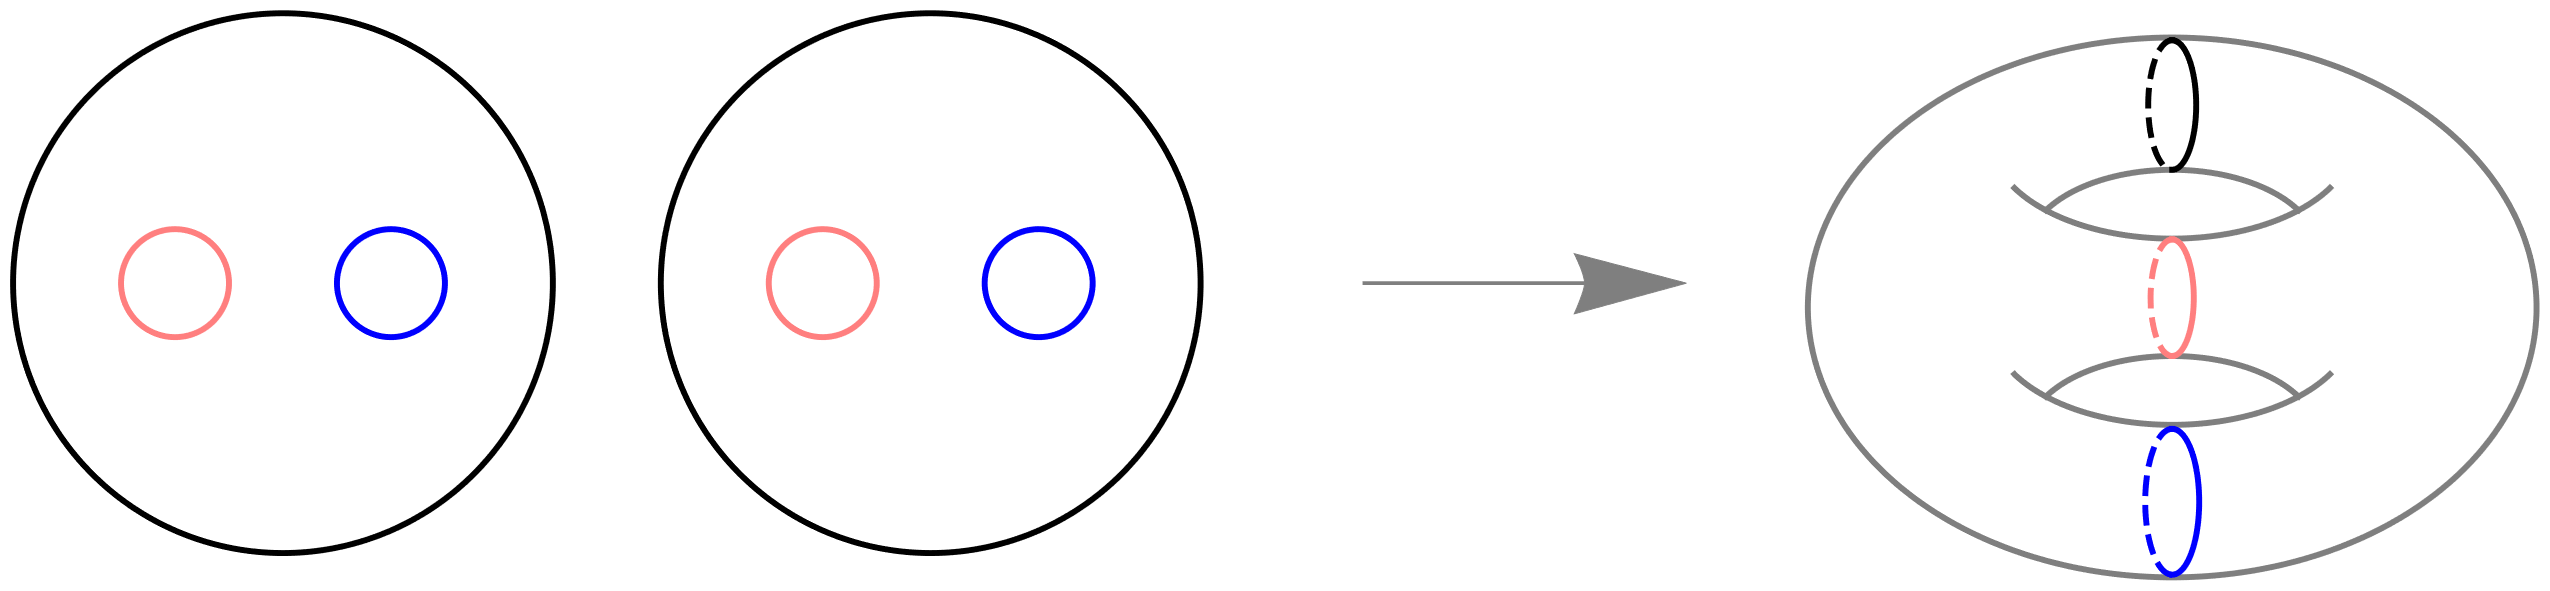
\includegraphics[width=0.85\textwidth]{figures/fig04.png}
  \caption{亏格 2 黎曼面的管道化构造：两个三孔球面（左、中）经三根管道（右）粘合；三根管道正对应 $3g-3=3$ 个复模。（原文 p.7，图 4）}
  \label{fig:4}
\end{figure}
% [Tutor Note: 数目要与图 4 对照看：$g=2$ 时 $2g-2=2$ 个三孔球面、$3g-3=3$ 个管道化映射，图 4 右侧就是两个三孔球面之间连三根管道。$3g-3$ 同时是亏格 $g$ 黎曼面模空间的复维数，故每根管道恰好贡献一个复模 $q$；$g=1$ 时 $3g-3=0$，只余一个复模 $\tau$，与环面情形相符。]

管道化构造给出一种精确的办法，在任意亏格 $g$ 的黎曼面上构造配分函数，更一般地构造关联函数。出发点是黎曼球面上任意 Virasoro 后代的三点函数，而三点函数由共形 Ward 恒等式用结构常数 $C_{ijk}$ 确定。所谓模不变性，就是断言：同一（带穿孔的）黎曼面的所有可能管道化构造，都给出相同的配分函数（关联函数）。

同一黎曼面的不同管道化构造之间等价，只需以下两条成立：所有球面四点函数都能等价地在两个不同通道中分解；由带一个穿孔的圆环内外边界管道化得到的全部环面一点函数，与把环面剪开成圆环的方式无关。前者正是前面已经提到的 OPE 结合性；后者等价于所有原初算符的环面一点函数具有模协变性。具体说来，对每个原初算符 $\phi_k(z,\bar z)$，环面一点函数 $\langle\phi_k(z,\bar z)\rangle_{T^2(\tau)}=f_k(\tau,\bar\tau)$ 是权为 $(h_k,\tilde h_k)$ 的模形式。也就是说，
\begin{equation}
  \label{eq:2-26}
  f_k(\tau+1,\bar\tau+1)=f_k(\tau,\bar\tau),\qquad
  f_k(-1/\tau,-1/\bar\tau)=(-i\tau)^{h_k}(i\bar\tau)^{\tilde h_k}f_k(\tau,\bar\tau).
\end{equation}
% [Tutor Note: (2.26) 是权 $(h_k,\tilde h_k)$ 模形式的定义：$T:\tau\to\tau+1$ 下不变，$S:\tau\to-1/\tau$ 下带自守因子 $(-i\tau)^{h_k}(i\bar\tau)^{\tilde h_k}$。环面一点函数与插入点 $z$ 无关，是因为环面上的平移 Killing 矢量使 $\langle\phi_k(z)\rangle$ 为常数，这对原初场成立。$S$ 变换中 $(-i\tau)^{h_k}$ 的 $i$ 相位与幂次是这一段里最易写错处，务必与 $q=e^{2\pi i\tau}$ 的约定一起核对。]
